\newcommand{\usecase}[8]
{
{
\small \begin{longtable}{@{}p{.2\textwidth}p{.01\textwidth}p{.79\textwidth}@{}}
\toprule Name & & \textbf{#1} \\
\midrule Goal & & #2 \\
\midrule Actor & & #3 \\
\midrule Pre-Condition & & #4 \\
\midrule Post-Condition & & #5 \\
\midrule Post-Condition in Special Case & & #6 \\
\midrule Normal Case & \multicolumn{2}{p{.8\textwidth}}{\vspace*{-0.5cm}#7} \\
\midrule Special Cases &  \multicolumn{2}{p{.8\textwidth}}{\vspace*{-0.5cm}#8} \\
\bottomrule
\caption[Description of Use Case: #1]{Description of Use Case \term{#1}.}
\end{longtable}
}
\label{table:#1}
\clearpage
}


\section{Use Cases}
\label{sec:usecases}

In this section we extend the tenant operator use cases which are described in Muhler's and Uralov's approach \cite{Muhler2012}, \cite{Uralov2012}. The tenant operators are the users with less permissions in JBIMulti2, who perform service registration and endpoint configuration operations in ServiceMix-mt. An overview of the set of use cases for the tenant operators is presented in Figure \ref{fig:usecases}. The set of use cases we add to the previous version are highlighted, and described in detail. 

\begin{figure}[htb]
	\centering
		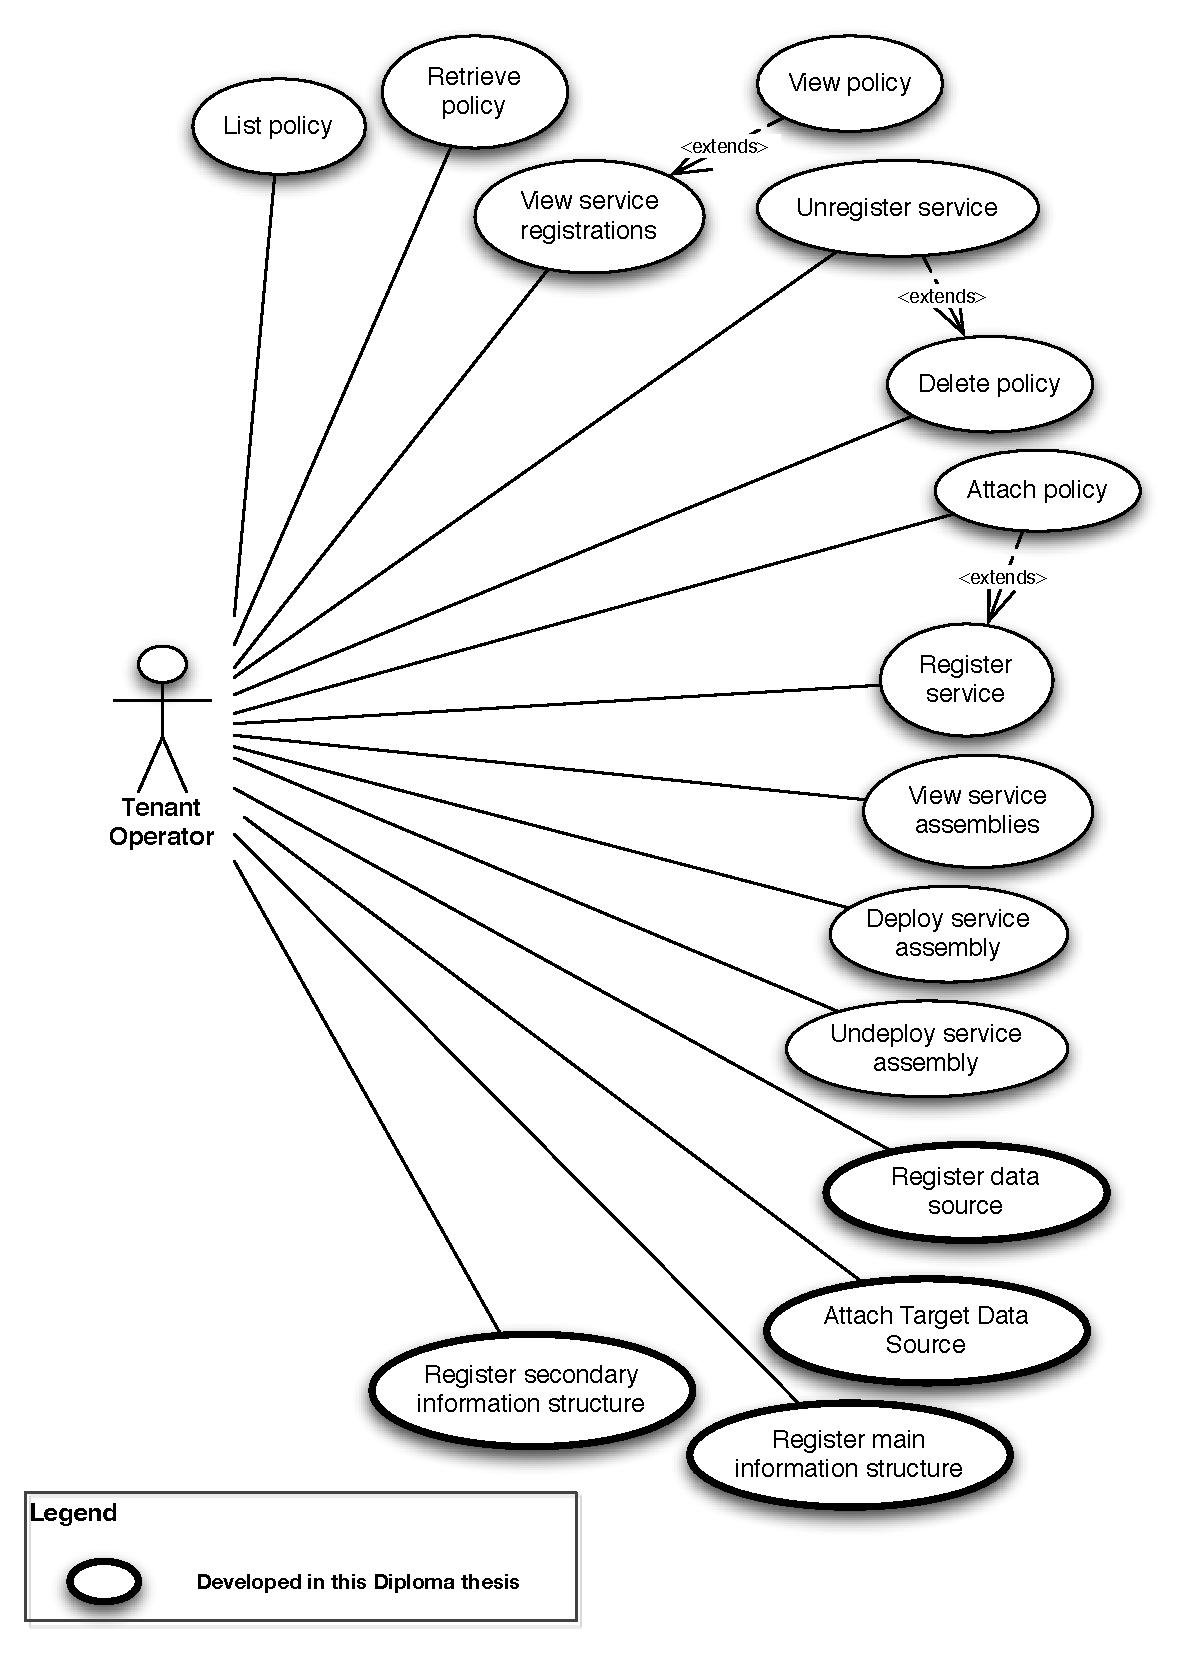
\includegraphics[clip, scale=0.59]{./gfx/usecaseDataSource.pdf}
	\caption[Use Case Diagram for Tenant Operator]{Use case diagram for tenant operator.}
	\label{fig:usecases}
\end{figure}

\pagebreak
\usecase{Register Data Source}
{The tenant operator wants to register a source and backend data source configuration data and associate it to an existing service assembly.}
{Tenant Operator}
{The tenant operator has the permissions in the service unit contingent and has registered a service assembly with no datasources associated to it.}
{Source and backend data source configuration data is stored successfully, and associated with a tenant's operator service assembly.}
{Source and backend data source configuration data are not stored, and not associated with the specified service assembly.}
{\begin{enumerate}
	\item The tenant operator selects the service assembly to which the data sources are associated.
	\item The source and target data sources configuration data are registered in the system, and associated to the specified service assembly.
\end{enumerate}}
{\begin{enumerate}
	\item[1a.] The service assembly does not exist.
		\begin{enumerate}
			\item The system shows an error message and aborts.
		\end{enumerate}
	\item[2a.] The service assembly is already associated with a source data source.
		\begin{enumerate}
			\item The system shows an error message and aborts.
		\end{enumerate}
	\item[2b.] The source data source configuration data already exists.
		\begin{enumerate}
			\item The system shows an error message and aborts.
		\end{enumerate}
	\item[2c.] The target data source configuration data already exists.
		\begin{enumerate}
			\item The system shows an error message and aborts.
		\end{enumerate}
\end{enumerate}}

\usecase{Attach Target Data Source}
{The tenant operator wants to attach one backend data source configuration data and associate it to an existing service assembly and source data source.}
{Tenant Operator}
{The tenant operator has the permissions in the service unit contingent and has registered a source data source.}
{The target data source is attached successfully to the specified source data source, and associated with the specified service assembly.}
{Target data source configuration data is not attached, and not associated with the specified service assembly.}
{\begin{enumerate}
	\item The tenant operator selects the service assembly to which the source data source is associated.
	\item The tenant operator selects the source data source to which the target data source must be associated.
	\item The target data source configuration data is attached to the specified source data source, and associated to the specified service assembly.
\end{enumerate}}
{\begin{enumerate}
	\item[1a.] The service assembly does not exist.
		\begin{enumerate}
			\item The system shows an error message and aborts.
		\end{enumerate}
	\item[2a.] The source data source does not exist.
		\begin{enumerate}
			\item The system shows an error message and aborts.
		\end{enumerate}
	\item[3a.] The target data source already exists.
		\begin{enumerate}
			\item The system shows an error message and aborts.
		\end{enumerate}
\end{enumerate}}

\usecase{Register Main Information Structure}
{The tenant operator registeres a main information structure and associate it with the specified source and target data source.}
{Tenant Operator}
{The tenant operator has the permissions in the service unit contingent and has registered the specified source and target data source.}
{The source and target main information structure meta-data is registered successfully, and associated with the specified source and target data source.}
{Source and target main information structure are not registered, and are not associated with the specified source and target data source.}
{\begin{enumerate}
	\item The tenant operator selects the service assembly to which the source data source is associated.
	\item The tenant operator selects the source and target data source to which the source and target main information structure is associated.
	\item The source and target main information structure are registered and associated with their source and target data source.
\end{enumerate}}
{\begin{enumerate}
	\item[1a.] The service assembly does not exist.
		\begin{enumerate}
			\item The system shows an error message and aborts.
		\end{enumerate}
	\item[2a.] The source or target data source does not exist.
		\begin{enumerate}
			\item The system shows an error message and aborts.
		\end{enumerate}
	\item[3a.] The main source or target information structure already exists.
		\begin{enumerate}
			\item The system shows an error message and aborts.
		\end{enumerate}
\end{enumerate}}

\usecase{Register Secondary Information Structure}
{The tenant operator registeres a secondary information structure and associates it with the specified source and target main information structure.}
{Tenant Operator}
{The tenant operator has the permissions in the service unit contingent, has registered a source and target data source, has registered a source and target main information structure, and the source and target datasources are \ac{NoSQL} databases.}
{The source and target secondary information structure meta-data are registered successfully, and associated with the specified source and target main information structure.}
{Source and target secondary information structure are not registered, and are not associated with the specified source and target main information structure.}
{\begin{enumerate}
	\item The tenant operator selects the service assembly to which the source data source is already associated.
	\item The tenant operator selects the source and target data source to which the main information structure are associated.
	\item The tenant operator selects the source and target main information structure to which the secondary information structure is associated.
	\item The source and target secondary information structure are registered and associated with their source and target main information structure.
\end{enumerate}}
{\begin{enumerate}
	\item[1a.] The service assembly does not exist.
		\begin{enumerate}
			\item The system shows an error message and aborts.
		\end{enumerate}
	\item[2a.] The source or target data source does not exist.
		\begin{enumerate}
			\item The system shows an error message and aborts.
		\end{enumerate}
	\item[2b.] The source and target data source is a MySQL database.
		\begin{enumerate}
			\item The system shows an error message and aborts.
		\end{enumerate}
	\item[3a.] The main source or target information structure does not exist.
		\begin{enumerate}
			\item The system shows an error message and aborts.
		\end{enumerate}
	\item[4a.] The secondary source or target information structure already exists.
		\begin{enumerate}
			\item The system shows an error message and aborts.
		\end{enumerate}
\end{enumerate}}



\FloatBarrier